\documentclass[a4paper,oneside,12pt]{book}
%% === nezbytné balíčky:
\usepackage[IL2]{fontenc}   % font for UTF-8 || other: [T1] (works for UTF-8?)
\usepackage[utf8]{inputenc} % input archive UTF-8 || [cp1250] -> Windows 1250 || [latin2] -> ISO Latin 2

\usepackage[english]{babel} % english wrote work, typographical rules     

\usepackage{pdfpages} % package allows to use pdf file insertion. Used to insert zadani_cele.pdf

\usepackage[a4paper, hmarginratio=1:1]{geometry} % usage of full A4 document page and frame limit - for two sided printing

%% === suitable packages
\usepackage[hidelinks]{hyperref} % a package - there will be clickable links in the PDF
\usepackage{graphicx} % a package for the insertion of RASTER graphics (PNG, etc.)
\usepackage{epsfig} % a package for the insertion of EPS-type VECTOR graphics files

\usepackage{float} % extended image location options
\usepackage{caption} % for the description of pictures, tables, etc.

\usepackage{tabularx} % extended table options
%\usepackage{tabu} % other package for extended spreadsheet options


\usepackage{listings}  % Package suitable for code samples 
\usepackage{amsmath} % the advanced mathematical rate package
%\usepackage{color} % for the possibility of coloured text
%\usepackage{fancybox} % Allows for advanced framing
%\usepackage{index} % to be used in case of makeindex registry creation. !!READ NEXT LINE
%\newindex{default}{idx}{ind}{Rejstřík} % establishes a register in the case of the use of an index package

%By me
\usepackage{fixltx2e} %Allows to use subscript for text

\topmargin=-15mm      % the upper edge slightly smaller
\textwidth=150mm      % width of the text on the page
\textheight=240mm     % 'height' of the text on the page

\nonfrenchspacing % In english texts space after sentence is bigger
\widowpenalty=1000 % "power" of the widow ban (= one line of paragraph at the bottom of the page)
\clubpenalty=1000 % "power" orphan ban (= one line/word paragraph separately at the top of the page)
\brokenpenalty=1000 % "power" ban of breaking the page after a line which has a split word at the end

\pagenumbering{arabic} % page numbering by Arabic numerals
\pagestyle{plain}      % pages numbered from the bottom to the middle

\parindent=0pt % deleting the first line of paragraph 1
\parskip=7pt   % gap between paragraphs

\newcommand{\ti}{\textit} % abbreviated command for italics
\newcommand{\tb}{\textbf} % abbreviated command for bold


%%-- there are macros, or "constants"-- some of them are necessary to be changed! --- %%
\newcommand{\cvut}{Czech Technical University in Prague}
\newcommand{\fjfi}{Faculty of Nuclear Sciences and Physical Engineering}
\newcommand{\katedra}{ Department of Physics}
\newcommand{\program}{Nuclear and Particle Physics} % stud. program
\newcommand{\spec}{--} % if a program has specialisation

\newcommand{\druh}{Bachelor's thesis}
\newcommand{\woman}{} % if a woman change to \newcommand{\woman}{a}

\newcommand{\logoCVUT}{
\includegraphics{symbol_cvut_konturova_verze_cb.pdf}} % the logo of the CTU -- according to the CTu graphic manual in force since December 2016. If the PDF-version does not fit, use another version of the logo: https://www.cvut.cz/logo-a-graficky-manual -> "Symbol and logo of the CTU in Prague"). If you want to omit the logo altogether, instead of "\includegraphics{...}" type the text "\vspace{35mm}"

% exactly according to the form 'Application for a Bachelor's degree/degree':
\newcommand{\nazevcz}{Tvrdé sondy ve vysokoenergetických srážkách na RHIC}    % Czech job title (according to the assignment!)
\newcommand{\nazeven}{Hard probes in high energy collisions at RHIC}          % English job title (according to the assignment!)
\newcommand{\autor}{Nikolai Denisov}
\newcommand{\vedouci}{Dr. Barbara Antonina Trzeciak, Ph.D.} % the name and surname of the supervisor of the work, including titles, e.g.: Doc. Ing. Ivo Malý, Ph.D.
\newcommand{\pracovisteVed}{\cathedra, \FNSPE, \CTU}
\newcommand{\konzultant}{--} % If there is a designated consultant, enter his name + titles
\newcommand{\pracovisteKonz}{--} % If there is a designated consultant, enter his work place

% Fill accordingly:
\newcommand{\rok}{2024}  % year of submission (only the year of submission, not the entire academic year!)
\newcommand{\kde}{Prague}

\newcommand{\klicova}{Klíčová slova}   % Here type in czech about 3-5 keywords !ASK
\newcommand{\keyword}{Key words}       % here type in English about 3-5 key words (translate from Czech, but professionally)

\newcommand{\abstrCZ}{Thesis description in Czech}    % Write abstract in Czech (at least 7 sentences, min. 80 words) here. Ensure that both the CZ and EN abstracts do not cause page 6 to overflow to page 7, i.e. that both with keywords fit on ONE page) !ASK
\newcommand{\abstrEN}{Thesis description in English} % Write abstract in English !ASK

\newcommand{\prohlaseni}{I declare that I have prepared my thesis on my own and have used only the materials (literature, projects, etc.) listed in the attached list.}

\newcommand{\podekovani}{Thanks you... for...} % WRITE a thank-you note, for example to your supervisor !ASK


\begin{document}
%%%%%%%%%%% TITLE -- the next 30 or so lines are generated AUTOMATICALLY. Do not change!!! Exception: papers written in English! %%%%%%%%%%%%
    \thispagestyle{empty}

    \begin{center}
    {\Large \textsc{\cvut}\\[4mm] \textsc{\fjfi}}\par
    \vspace{4mm}
    \tb{\katedra} \par\vspace{3mm}

    \begin{tabular}{l}
        \tb{Study program: \program}\\
        \tb{Specialization: \spec}\\
    \end{tabular}

    \vspace{10mm} \logoCVUT \vspace{15mm}

    {\huge \tb{\nazevcz}\par}
    \vspace{5mm}
    {\huge \tb{\nazeven}\par}

    \vspace{15mm}
    {\Large \MakeUppercase{\druh}}

    \vfill
    {\large
        \begin{tabular}{ll}
            Produced by: & \autor\\
            Supervisor: & \vedouci\\
            Year: & \rok
        \end{tabular}
    }
    \end{center}

%%%%%%%%%%%% ZADÁNÍ PRÁCE %%%%%%%%%%%%
% Zadání (podepsané děkanem atd.) dostanou studenti KSI od sekretářky (nebo ji požádají, např. e-mailem).
    \newpage  % SEM NESAHEJTE!
    \thispagestyle{empty} % SEM NESAHEJTE!

    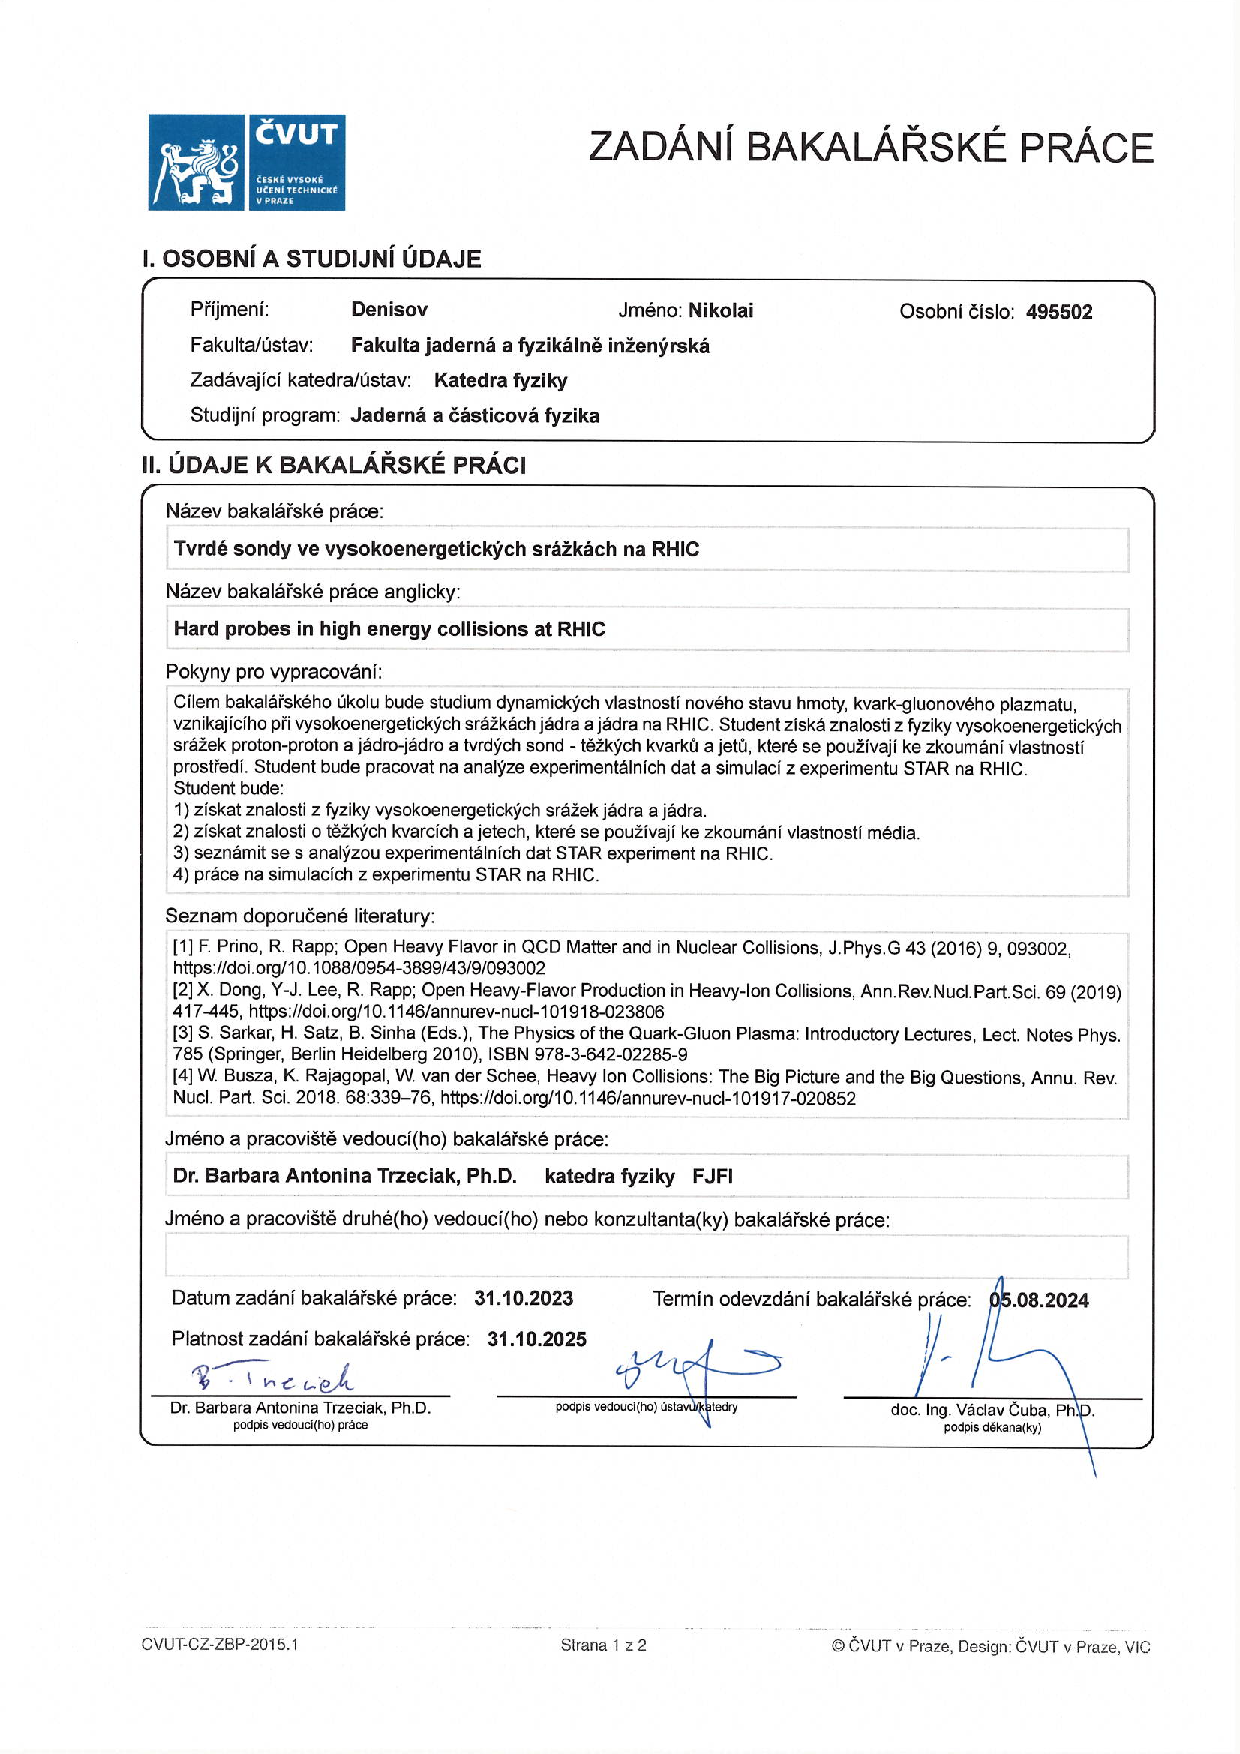
\includepdf[pages={1,2}]{zadani_cele.pdf} % PDF má 2 stránky



%%%%%%%%%%%% Prohlášení -- SEM NESAHEJTE! Generuje se automaticky z výše nastavených maker \kde{} a \prohlaseni{}. %%%%%%%%%%%%
    \newpage % SEM NESAHEJTE!
    \thispagestyle{empty}  % SEM NESAHEJTE!

    ~ % SEM NESAHEJTE!
    \vfill % prázdné místo. SEM NESAHEJTE!

    \tb{Declaration} % SEM NESAHEJTE!

    \vspace{1em} % vertikální mezera. SEM NESAHEJTE!
    \prohlaseni

    \vspace{2em}  % SEM NESAHEJTE!
    \hspace{-0.5em}\begin{tabularx}{\textwidth}{X c}  % SEM NESAHEJTE!
                       In \kde\  .................... &........................................ \\	% SEM NESAHEJTE!
                       & \autor
    \end{tabularx}	% SEM NESAHEJTE!


%%%%%%%%%%%% Poděkování -- tuto stránku můžete celou odstranit %%%%%%%%%%%%
    \newpage
    \thispagestyle{empty}

    ~
    \vfill % prázdné místo

    \tb{Poděkování}

    \vspace{1em} % vertikální mezera
    \podekovani
    \begin{flushright}
        \autor
    \end{flushright}  % <------- tady končí stránka s poděkováním


%%%%%%%%%%%% ABSTRAKT atp. Je generován AUTOMATICKY podle maker nastavených na začátku souboru) %%%%%%%%%%%% 
    \newpage   % SEM NESAHEJTE!
    \thispagestyle{empty}   % SEM NESAHEJTE!

% příprava:    (na následujících 8 řádků NESAHEJTE!)
    \newbox\odstavecbox
    \newlength\vyskaodstavce
    \newcommand\odstavec[2]{%
        \setbox\odstavecbox=\hbox{%
            \parbox[t]{#1}{#2\vrule width 0pt depth 4pt}}%
        \global\vyskaodstavce=\dp\odstavecbox
        \box\odstavecbox}
    \newcommand{\delka}{120mm} % šířka textů ve 2. sloupci tabulky

% použití přípravy:    % dovnitř "tabular" vůbec NESAHEJTE!
    \begin{tabular}{ll}
    {\em Název práce:} & ~ \\
    \multicolumn{2}{l}{\odstavec{\textwidth}{\bf \nazevcz}} \\[1em]
    {\em Autor:} & \autor \\[1em]
    {\em Studijní program:} & \program \\
    {\em Specializace:} & \spec \\
    {\em Druh práce:} & \druh \\[1em]
    {\em Vedoucí práce:} & \odstavec{\delka}{\vedouci} \\
    {\em Konzultant:} & -- %\odstavec{\delka}{\konzultant \\ \pracovisteKonz}  % VYMAŽTE text "-- %" v případě, že jste neměli konzultanta
    \\[1em]
    \multicolumn{2}{l}{\odstavec{\textwidth}{{\em Abstrakt:} ~ \abstrCZ  }} \\[1em] %WRITE ABSTARCAT
    {\em Klíčová slova:} & \odstavec{\delka}{\klicova} \\[2em]
    %WRITE KEY WORDS
    {\em Title:} & ~\\
    \multicolumn{2}{l}{\odstavec{\textwidth}{\bf \nazeven}}\\[1em]
    {\em Author:} & \autor \\[1em]
    \multicolumn{2}{l}{\odstavec{\textwidth}{{\em Abstract:} ~ \abstrEN  }} \\[1em]
    {\em Key words:} & \odstavec{\delka}{\keyword}
    \end{tabular}



%%%%%%%%%%%% Obsah práce ... je generován AUTOMATICKY %%%%%%%%%%%%
    \newpage  % SEM NESAHEJTE!
    \parskip=0pt
    \tableofcontents % SEM NESAHEJTE!
    \parskip=7pt
    \newpage % SEM NESAHEJTE!


%--------------------------------------------------------
%|         Here starts the thesis (text)              |
%--------------------------------------------------------

    \chapter{Introduction} %add quark guon plasma, phase diagram, probbing with focus on jets and heavy flavour
    \section{General description} %, rapidity, time-space diagram, jet variables, CAN't BE LIKE THAT MUT BE MORE DESCIBETIVE
    \section{Physics of the particle collisions}
    \section{Current results on heavy flavour jet angularities} %describe results from ALICE
    \section{RHIC and STAR}



    \chapter{Jet algorithms} %brief description
    \section{k\textsubscript{t} algorithm}
    \section{anti-k\textsubscript{t} algorithm}
    \section{Cambridge-Aachen algorithm} %brief
    \section{SISCone Algorithm algorithm} %brief


    \chapter{Simulations of hard probes in high energy collisions}
    \section{Pythia}
    \section{STAR and RHIC settings}
    \section{Simulation results} %algorithms comparision, basic distributions with star requirments

    \chapter{Heavy flavour jets simulations for STAR}
    \section{D\textsubscript{0} jet tagging}
    \section{Variables}









    \chapter*{Conclusion} %What have been simulated, for what and why Pythia is good for that

    \addcontentsline{toc}{chapter}{Conclusion}

%%%%%%%%%%%% The list of used sources (LITERATURE) %%%%%%%%%%%% !ASK IF IT IS POSSIBLE TO ADD PRESENTAtIONs -> NO, but I can make reference to one of the books 
    \clearpage
    \addcontentsline{toc}{chapter}{The list of used sources}
    \begin{thebibliography}{99}
% replace the following text (2 lines) with citations of your sources
        \bibitem{odkaz} Autor. \ti{Název knihy}. Město. Nakladatelství. Rok.
    \end{thebibliography} %ADD GITHUB HERE
% the following format: CN ISO 690. You can generate it at http://www.citacepro.com (sign in via the "CITATES" link), it can generate TeX
% order: alphabetically by author (or by first name, if author is unknown)


    \newpage
    \addcontentsline{toc}{chapter}{Apendix} % Pythia settings for visualisation, for STAR, for D_0 jets, additional plots. NO CODE
    \appendix

    \chapter{Apendicies' name} % here change the name of the annex, or comment and insert the file where the name of the annex is + its text (delete/comment the text below + uncomment \input{}):

\end{document} % End.
